\section{Addressing Storage and Bandwidth Limitations}
\label{sec-prioritylance}

The simple event-based triggering we deployed at Reventador volcano in 2005
displayed a number of weaknesses that had to be addressed in order to build a
more scalable system.  In particular, these limitations led to significant
loss of data and the overall approach would not have scaled as the size of
the network or the lifetime target increased.  After analyzing the
performance of the 2005 network we identified three key weaknesses:

\begin{enumerate}
\item \textbf{Lack of Data Prioritization:}Our event-triggered system
attempted to download data corresponding to well-correlated seismic events.
However, the event detector operated in a binary fashion, leaving it unable
to prefer certain events over others.  Because we required each node to make
an individual, local decision as to what constituted an ``interesting''
event, the efficacy of the system as a whole was largely dependent on this
parameter. After analyzing the data collected at Reventador we determined
that the original threshold was likely set far too low, causing our network
to trigger on less than 5\% of the actual seismic events observed by wired
stations during the deployment. Without the ability to prioritize events
setting a threshold means either risking underutilization if the threshold is
too high or being unable to distinguish between extremely-interesting and
less-interesting triggers if it is too low.

\item \textbf{FIFO Storage Management:} Due to the limited flash storage
available on each TMote Sky, each node could only store around 20~minutes of
continuous sensor data.  When an interesting event occurred, to avoid
overwriting data about to be requested for download we disabled sampling on
each node until the data corresponding to the event in question had been
downloaded.  Due to the high download latency imposed by reliable transfer
over multiple lossy links, and the high event frequency, a large portion of
the network was offline for a significant amount of time after each triggered
seismic event. This led to data loss.

\item \textbf{FIFO, Non-Preemptive Download Policy:} Following each triggered event
we downloaded signals from each node in turn until the entire event was
captured. As previously mentioned, this download process took a significant
amount of time during which many nodes were not sampling. This meant that
smaller, less interesting events could prevent the detection of larger,
potentially more interesting ones if the small event occurred slightly
earlier in time, since the network would still be busy downloading the small
event when the large event occurred.  Given that many large eruptions are
preceded by small precursor earthquakes, this meant that many such large
events failed to be recorded at all.
\end{enumerate}

As an initial response to these challenges we developed a utility-driven
architecture for optimizing the value of downloaded data in the face of
storage and bandwidth constraints.  Putting aside the datum quality issues
this architecture attempts to address dataset quality directly by allowing
the application to express preferences for some data over others and having
the system attempt to maximize the value of the downloaded data while meeting
constraints on storage, bandwidth, energy and target lifetime.  Based on
experiences with earlier systems the design of a new system, Lance, was
guided by several overarching design principles:

\begin{enumerate}
\item \textbf{Decouple mechanism from policy.} When possible we wanted to begin to
abstract the development of our approaches to dataset problem away from the
volcano application context, making Lance suitable for use in multiple
application domains.
\item \textbf{Simplicity through centralized control.} As previously described, we
had significantly simplified the design of our volcano-monitoring network
by aggregating functionality on the base station. Lance continues this
approach, again treating nodes as slave devices.
\item \textbf{Low overhead for maintenance traffic.} The drawback of a centralized
solution can be high overhead for the associated control and maintenance
traffic. We wanted to avoid this if possible by dividing decision making
between local per-node components and global components running at the base
station and optimizing the communication patterns between the two.
\end{enumerate}

This architecture developed through two iterations, the second of which was
published as Lance~\cite{lance-sensys08}.  The first and second version of
this system share a policy module architecture allowing applications to
tailor the data collection strategy. The two iterations differ, however, in
significant ways, with most of the changes resulting from our 2007 deployment
at Tungurahua Volcano.  The first system presents an \textit{ordinal}
(ordering-only) conception of utility, addresses storage and bandwidth as
constraints, and attempts to maximize the value of the collected data without
considering cost. The second moves to a \textit{cardinal} (ordering and
exchange) conception of utility, focuses on energy and bandwidth as
constraints, and develops and deploys a cost model as part of the
maximization process.  This and the two sections that follow place these
efforts into the broader context of an approach to dataset quality.

\subsection{Overview of Lance}

\begin{figure}[t!]
\begin{center}
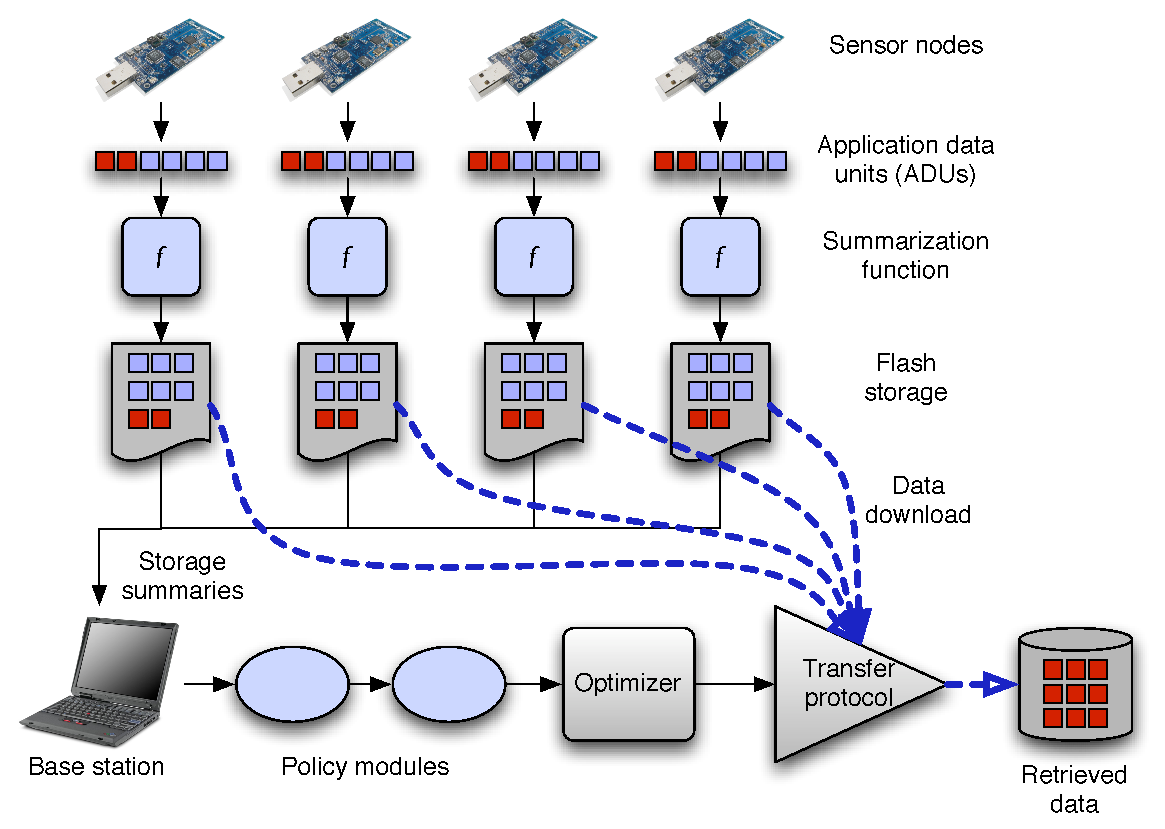
\includegraphics[width=1.0\hsize]{./figs/Sensys2008/2008-lance-architecture.eps}
\end{center}
\caption{{\bf Lance architecture.}
The architecture of both the priority- and utility-driven versions of
Lance is quite similar. The interpretation of the assigned utility values
differs, but the major architectural components are the same.}
\label{fig-lance-architecture}
\end{figure}

Figure~\ref{fig-lance-architecture} provides an overview of the Lance
architecture. Sensor nodes sample sensor data, storing the data to local
flash storage. Each application data unit (ADU) consists of some amount of
raw sensor data, a unique {\em ADU identifier}, and a {\em timestamp}
indicating the time that the first sample in the ADU was sampled. ADU
timestamps can either be based on local clocks at each node, or tied to a
global timebase using a time synchronization protocol such as
FTSP~\cite{ftsp}. The size of an ADU should be chosen to balance the
granularity of data storage and download with the overhead for maintaining
the per-ADU metadata. In the applications we have studied, an ADU stores
several seconds or minutes of sensor data, not an individual sample. ADUs are
stored locally in flash, which is treated as a circular buffer.

Ideally, nodes would be able to compute the value $v_i$ of an ADU locally, as
the data is sampled. However, since the value might depend on factors other
than the ADU's data, such as data computed at other nodes. Lance assigns
values $v_i$ at the base station, based on global knowledge of the state of
the network. However, this requires nodes to communicate some low-bandwidth
information on the ADU contents to the base station.  For this purpose, each
node applies an application-supplied {\em summarization function}, computing
a concise summary $s_i$ of the contents of the ADU as it is sampled.  Nodes
periodically send {\em ADU summary} messages to the base station, providing
information on the ADUs they have sampled, their summaries, timestamps, and
other metadata. As a special case, if a node is able to assign the ADU's
initial value directly, this is used as the summary.

The Lance {\em controller} receives ADU summaries from the network.  The
controller also estimates the download cost $\bar{c}_i$ for each ADU, based
on information on network topology as well as a model of energy consumption
for download operations. The ADU summaries and cost are passed through a
series of {\em policy modules}, which provide application-specific logic to
assign the value $v_i$ to each ADU.  The resulting values are passed to the
Lance {\em download manager} which is responsible for performing downloads,
using a reliable data-collection protocol, such as
Flush~\cite{flush-sensys07}.

\subsection{Cardinal v Ordinal Utilities}

One significant difference between the first and second versions of Lance is
the meaning of the utility values assigned to each ADU.  Utility values
assigned to each ADU are intended to reflect the value of that signal to the
application, with higher utilities indicating more valuable data.  Accurate
and efficient utility assignment -- while a difficult and
application-specific challenge -- is crucial to the Lance approach.

The first version used \textit{ordinal} utilities (or priorities), meaning
that the assigned utilities established an order among available ADUs but did
not reflect the relative importance of one ADU versus another. Given
priorities, an ADU assigned priority 100 can only be assumed to me more
valuable that one assigned an ADU 99. It might be 100 times more valuable. It
might be only 2 times more valuable.  The fact that ordinal utilities produce
a strict ordering and nothing else simplified the policies of the first
system. The storage manager could easily prioritize available flash on each
node, and the download manager simply downloaded the available ADU with the
highest utility, irregardless of the resources necessary to do so. Since
ordinal utilities do not allow the value of an ADU to be weighed against the
cost (in system resources) required to download it, they render the notion of
cost unnecessary.

The second iteration of Lance used \textit{cardinal} utilities, which not
only produce an ordering but also imply relative value between ADUs. So an
ADU assigned utility 100 is assumed to be twice as valuable as one assigned
utility 50. This formulation allows the incorporation of cost into the
optimization framework, as described later in Sect.~\ref{sec-lance}.

\subsection{Utility Functions}

Implicit in Lance is the idea that, when addressing dataset quality, wheat
must be separated from chaff. We rely on a utility function to do so,
irregardless of whether the utility is interpreted as a cardinal or ordinal
one.  In general utility functions can be quite complex, depending not only
on the data acquired at a particular node but also on the distribution of
data across the network, availability of storage, bandwidth, energy and other
resources, and so forth.  To help designers construct complete systems
\textit{without} starting from scratch, Lance attempts to cleanly separate
the \textit{policies} governing how to divide data into interesting and
uninteresting piles from the \textit{mechanisms} governing the collection of
data after the division is performed.

To leverage global knowledge while reducing the resource consumption on each
node, we separate local knowledge from global by effectively diving the
utility assignments between node-specific (the utility calculator that runs
on each node) and network-wide (the policy module chain described in the next
section) components.  The node-level utility calculator operates only based
on inputs available on a single node and must run on a resource-constrained
sensor network node, limiting the amount of computation it can perform.  In
contrast, the network-wide policy modules running on the powered base station
have access to a global view of the network and significantly augmented
resources. As such they can use global, historical and out-of-band
information to further refine the initial utility assignment performed on the
node itself.

Communication between the node-level and network-wide portions of the utility
function is overhead with respect to the application goals, and so a
practical requirement limiting the usage of Lance is keeping the traffic
between these two components to a minimum. The utility functions we have
developed in the context of the volcano application have typically limited
this overhead by having the output of the node-level utility function be a
single scalar value, which can be efficiently transmitted to the base
station.  There is no requirement that the node-level utility function
produce such simple outputs, but it does aid in reducing the overhead
inherent in the utility assignment process.

As a concrete example tying Lance to previous work, the distributed event
detector deployed at Reventador in 2005 could be easily reimplemented in
Lance. The node-level utility calculator uses the ratio of two EWMAs to
assign a binary utility, either one or zero, to each ADU. At the network
level, a policy module aggregates these assignments and, when enough overlap
within a particular time window, it marks that entire segment of data with a
unit utility value (all other time windows receive utility zero). Because
each ``interesting'' set of signals receives the same utility value, Lance
does not distinguish between them and will download them in a LIFO fashion.

\subsection{2007 Deployment}

To evaluate the performance of Lance in a real field setting, we undertook a
one week deployment of eight~sensor nodes at Tungurahua Volcano, Ecuador, in
August~2007. The priority-driven version of Lance was used to manage the
bandwidth resources of the sensor network, as described below. Time and
budget constraints prevented us from deploying a larger network for longer
period of time. Our primary goal was to validate Lance's operation in a field
campaign, as well as to identify challenges that only arise in real
deployments. Our experiences during this deployment led to further
refinements of Lance described in the next section.

\begin{figure}[t!]
\caption{{\bf Download performance during the deployment.}}
\vspace{0.2in}
\begin{center}
\begin{tabular}{lll}
\noalign{\smallskip}
{\bf Node}	& {\bf ADUs downloaded} & {\bf Mean throughput} \\
\noalign{\smallskip}\svhline\noalign{\smallskip}
100 & 311 & 651.0 B/sec \\
101 & 131 & 446.8 B/sec \\
102 & 262 & 445.8 B/sec \\
103 & 292 & 424.4 B/sec \\
104 & 150 & 256.8 B/sec \\
105 & 66 & 453.7 B/sec \\
106 & 20 & 253.4 B/sec \\
\noalign{\smallskip}\svhline\noalign{\smallskip}
{\em Total} & 1232 & 431.5 B/sec \\
\end{tabular}
\end{center}
\label{fig-throughputtable}
\end{figure}

The sensor network was operational for a total of 71~hours, out of which the
Lance download manager ran for a total of 56~hours.  During this time, Lance
successfully downloaded 1232~ADUs, or 77~MB of raw data. An additional
308~downloads failed due to timeout or stale summary information, for an
overall success rate of 80\%.  11012~unique ADU summaries were received from
the network, representing an aggregate of 688~MB of sampled data. Lance
therefore downloaded approximately 11\% of the data produced by the network.
Figure~\ref{fig-throughputtable} summarizes the number of ADUs downloaded
and the mean throughput for each node. 

\subsubsection{RSAM v EWMA Node Level Utility Calculator}
\label{subsubsec-rsamvewma}

The system as initially deployed computed the RSAM~\cite{rsam} (Reduced
Seismic Amplitude Measurement) as the value for each ADU.  This approach was
intended to prioritize data based on the overall level of seismic activity.
We experienced two problems as soon as the system was fielded. First, the
RSAM calculation was sensitive to DC~bias in the seismometer signal, causing
Lance to generally prefer downloading ADUs from one or two nodes (those with
the largest positive bias). We were able to work around this problem using
\textit{policy modules}, described in the next section.

The second problem with the RSAM utility calculator was caused by the
uncharacteristically low level of seismicity at the volcano throughout the
deployment. We observed only about 20~volcano-tectonic earthquakes and {\em
no} clear explosions, whereas the previous week, Tungurahua exhibited dozens
of earthquakes each day. As a result, the RSAM utility calculator was
generally unable to distinguish between actual seismic activity and noise.
Given the low level of volcanic activity, after the first 25~hours of the
deployment we chose to reprogram the network to use a different utility
calculator designed to pick out small earthquakes from background noise.  This
function computes the maximum ratio of two EWMA filters over the seismic
signal; it is similar to that described in~\cite{volcano-osdi06}. Due to code
size limitations on the motes, it was necessary to manually reprogram each
node with the new utility calculator, which took two teams about 4~hours.

We return to the 2007 deployment later in this chapter in two other contexts.
First, we discuss \textit{policy modules}, a useful feature that spanned both
the priority- and utility-driven versions of Lance.  We illustrate their use
with examples from our field deployment. Finally we present the mature,
utility-driven Lance, and also include an evaluation of its performance based
on data collected during our 2007 deployment.
